\section{Resultados dos Testes da Camada de Segurança (Ascon)}
\label{sec:resultados_ascon}

Esta seção reúne os resultados dos testes de validação e avaliação da camada de segurança baseada no Ascon, seguindo a metodologia definida na Seção \ref{subsec:validacao-ascon}. A camada de segurança atua sobre o \textit{payload} de cada mensagem antes de ele ser entregue ao rádio, e os resultados a seguir não dependem da configuração do enlace, tratada na Seção~\ref{sec:resultados_infra}. As condições em que eles valem estão reunidas na Seção~\ref{subsec:limitacoes_ascon}.

%%%%%%%%%%%%%%%%%%%%%%%%%%%%%%%%%%%%%%%%%%%%%%%%%%%%%%

\subsection{Validação por \textit{Known Answer Tests} (KAT)}
\label{subsec:kat_resultados}

A validação funcional foi conduzida com os vetores oficiais do Ascon-128a (versão 1.2) distribuídos com a \textit{ascon-suite}. Inicialmente, a biblioteca foi compilada em um computador \textit{desktop} e submetida à execução exaustiva dos 1089 vetores de teste, nos quais cada combinação de chave, \textit{nonce}, dados associados e texto em claro deve produzir um texto cifrado e uma \textit{tag} de autenticação exatos.

Todos os 1089 vetores foram processados com correspondência integral em relação às saídas esperadas, sem nenhuma falha. Como verificação adicional, os vetores foram regenerados a partir da própria implementação e comparados byte a byte com o arquivo de referência, resultando em arquivos idênticos. Por fim, a suíte de testes automatizados (\textit{CTest}) foi executada sobre as variantes em C, C++, \textit{SIV} e mascarada do algoritmo, com aprovação nos 14 casos avaliados. A Tabela~\ref{tab:kat_ascon128a} sintetiza esses resultados.

\begin{table}[htb]
\centering
\caption{Resultado da validação por \textit{Known Answer Tests} do Ascon-128a}
\label{tab:kat_ascon128a}
\begin{tabular}{lrr}
\hline
\textbf{Verificação} & \textbf{Casos} & \textbf{Falhas} \\
\hline
Execução exaustiva (\textit{desktop})                  & 1089 vetores & 0 \\
Regeneração \textit{vs.} referência                    & 1089 vetores & 0 \\
Suíte \textit{CTest} (C, C++, \textit{SIV}, mascarada) & 14 testes    & 0 \\
Execução na placa (ESP32, subconjunto)                 & 6 vetores    & 0 \\
\hline
\end{tabular}
\legend{Fonte: elaborado pelos autores.}
\end{table}

Esses resultados comprovam que a implementação do Ascon-128a opera corretamente no ambiente de desenvolvimento, reproduzindo de forma exata os valores de referência do algoritmo.

Confirmada a correção em \textit{desktop}, um subconjunto representativo dos vetores foi executado diretamente na placa ESP32, cobrindo os limites de processamento por blocos, com entrada vazia, bloco parcial, bloco completo e múltiplos blocos, com e sem dados associados. Para cada vetor, verificaram-se tanto a cifragem, comparando o resultado com o valor de referência, quanto a decifragem, confirmando a recuperação do texto claro com a \textit{tag} validada. Os seis vetores foram reproduzidos com correspondência integral na placa, descartando divergências introduzidas pela compilação ou pela arquitetura do \textit{hardware} (Xtensa LX, \textit{little-endian}). Nessa execução, o estado interno do algoritmo (\texttt{ascon128a\_state\_t}) ocupou 80 bytes, valor retomado posteriormente na análise de memória.

Os vetores utilizados e o registro completo das execuções, em \textit{desktop} e na placa, estão disponíveis no repositório do projeto, na pasta \texttt{kat-validation}.

%%%%%%%%%%%%%%%%%%%%%%%%%%%%%%%%%%%%%%%%%%%%%%%%%%%%%%

\subsection{Validação dos Dados Associados (AEAD)}
\label{subsec:aead_resultados}

A propriedade de autenticação do modo AEAD foi avaliada por injeção intencional de falhas, simulando um atacante que intercepta e altera a mensagem em trânsito. A partir de um pacote válido, cada adulteração foi aplicada isoladamente e a mensagem resultante submetida à decifragem, que deveria recusá-la.

A avaliação cobriu quatro frentes de adulteração. Às três previstas na metodologia, com texto cifrado, dados associados e \textit{tag} de autenticação. Acrescentou-se o \textit{nonce}, uma vez que, em um pacote real, ele trafega em claro junto da mensagem para que o destinatário possa decifrá-la, e portanto também está ao alcance do interceptador.

Além da inversão de um bit, aplicaram-se alterações que ela não alcança, inversão de dois bits simultâneos, inversão de um byte inteiro, substituição de um byte por zero, inversão de bits em posições distantes, truncamento, acréscimo de bytes ao final e reordenação de bytes adjacentes. Todas são exaustivas e deterministas, percorrendo posições fixas do pacote sem qualquer sorteio, de modo que a bateria é integralmente reproduzível.

O procedimento foi repetido em seis formatos de pacote, escolhidos sobre as fronteiras de bloco do algoritmo, que processa 128 bits por vez, com texto claro vazio, bloco parcial, bloco exato, bloco acrescido de um byte e múltiplos blocos, com e sem dados associados. Os subtotais por formato foram 602, 476, 786, 802, 1.063 e 1.178 adulterações. A Tabela~\ref{tab:aead_ascon128a} agrega os resultados por tipo de adulteração.

\begin{table}[htb]
\centering
\caption{Rejeição de adulterações no Ascon-128a, agregada em seis formatos de pacote}
\label{tab:aead_ascon128a}
\begin{tabular}{lrr}
\hline
\textbf{Adulteração} & \textbf{Casos} & \textbf{Rejeições} \\
\hline
\multicolumn{3}{l}{\textit{Inversão de um bit}} \\
\quad Texto cifrado (\textit{ciphertext}) & 784 & 784 \\
\quad Dados associados (AD)               & 928 & 928 \\
\quad \textit{Tag} de autenticação        & 768 & 768 \\
\quad \textit{Nonce}                      & 768 & 768 \\
\multicolumn{3}{l}{\textit{Demais alterações}} \\
\quad Dois bits simultâneos               & 776 & 776 \\
\quad Byte invertido                      & 194 & 194 \\
\quad Byte substituído por zero           & 194 & 194 \\
\quad Bits em bytes distantes             &  96 &  96 \\
\quad Truncamento do pacote               & 188 & 188 \\
\quad Acréscimo de bytes                  &  24 &  24 \\
\quad Reordenação de bytes                & 187 & 187 \\
\hline
Total                                     & 4.907 & 4.907 \\
\hline
\end{tabular}
\legend{Fonte: elaborado pelos autores.}
\end{table}

Como controle, o pacote intacto foi decifrado com sucesso em todos os seis formatos, recuperando o texto claro original. Nenhuma das 4.907 adulterações foi aceita, em todas, a decifragem reconheceu a quebra de integridade e retornou erro.

A metodologia exige que nenhum fragmento do texto claro seja entregue à aplicação. Para avaliá-la, o \textit{buffer} de saída foi preenchido, antes de cada decifragem, com um valor que não ocorre no texto claro. Após cada recusa, mediu-se a maior sequência de bytes presente simultaneamente no \textit{buffer} e no texto claro original. Em todas as 4.907 recusas, essa sequência foi de zero bytes, ou seja, não restou um único byte do texto claro. O mesmo procedimento aplicado ao pacote intacto recupera a mensagem integralmente, o que confirma que a verificação detectaria um vazamento caso houvesse.

A bateria foi executada em duas plataformas, o ESP32 clássico (Xtensa LX6) e o ESP32-S3 da placa Heltec (Xtensa LX7), e os resultados foram idênticos em todos os valores. A coincidência entre arquiteturas distintas indica que a rejeição de adulterações decorre do algoritmo, e não de particularidades de uma compilação ou de um \textit{hardware}.

Qualquer alteração da mensagem em trânsito, seja no \textit{payload}, nos metadados do cabeçalho, no \textit{nonce} ou na própria \textit{tag}, é portanto detectada e rejeitada sem vazamento de conteúdo, o que satisfaz o RF-S8 e confirma o emprego da \textit{tag} em seu comprimento integral exigido pelo RNF-S5, ambos especificados na Seção~\ref{sec:requisitos_seguranca}.

Cabe registrar o limite desta propriedade. O modo AEAD garante integridade, não frescor, um pacote válido capturado e retransmitido sem alteração alguma é aceito, pois de fato não foi adulterado. A detecção de repetição exige que o receptor mantenha registro do último \textit{nonce} aceito por dispositivo e recuse valores repetidos ou regressivos, o que pertence à camada de comunicação e não ao algoritmo. Esse tratamento é objeto do RF-S9, cuja verificação não integra os resultados desta seção.

O código de teste e os registros das execuções nas duas placas estão no repositório, na pasta \texttt{aead-validation}.

%%%%%%%%%%%%%%%%%%%%%%%%%%%%%%%%%%%%%%%%%%%%%%%%%%%%%%

\subsection{Consumo de Memória, Tempo de Execução e Tempo Constante}
\label{subsec:memoria_tempo}

As medições desta seção e da seguinte foram obtidas com um único \textit{firmware} de teste, executado em duas placas, o ESP32 clássico (Xtensa LX6), usado nas etapas anteriores, e o ESP32-S3 da placa Heltec WiFi LoRa 32 V3 (Xtensa LX7), que é a plataforma de implantação. Ambas operaram a 240~MHz, com \textit{firmware} compilado pelo \textit{core} arduino-esp32 3.3.11 sobre o ESP-IDF 5.5.5. Antes de qualquer medição, ele executa dois vetores do KAT oficial do Ascon-128a e um vetor de referência do AES-GCM, cifrando, decifrando e recusando uma \textit{tag} adulterada, e uma falha interromperia a execução, como prevê a Seção~\ref{subsec:validacao-ascon}. Os tamanhos de \textit{payload} foram 0, 2, 16, 23, 32 e 64 bytes. Os múltiplos de 16 sustentam o modelo de custo por bloco, o \textit{payload} vazio mede a parcela fixa diretamente, e 2 e 23 bytes são os dois tamanhos que ocorrem no \textit{dataset} Tour Perret, usado pela frente de aprendizado de máquina, em que 91\% das mensagens têm 23 bytes e 7\% têm 2 bytes \cite{tourperret_dataset}. O \textit{firmware}, os registros das duas placas e o programa que gera as tabelas e figuras estão na pasta \texttt{benchmark-validation/Ascon128a\_Benchmark\_Suite} do repositório.

Quanto à memória, a cifragem e a decifragem do Ascon-128a não realizaram nenhuma alocação dinâmica em nenhum dos seis tamanhos, nas duas placas. Como uma alocação feita e liberada dentro da operação não apareceria numa comparação antes e depois, o \textit{heap} livre foi lido continuamente durante cada operação por uma tarefa no outro núcleo do processador, e o menor valor observado coincidiu com o inicial em todos os casos. O mesmo procedimento aplicado ao AES-128-GCM mostrou que, no ESP32-S3, o \textit{driver} do ESP-IDF aloca e libera 40 bytes a cada chamada, por causa dos descritores da transferência por DMA \cite{espressif2026idf}. No ESP32 clássico, cujo \textit{driver} não usa DMA, não houve alocação. O resultado atende ao RNF-S6 para o Ascon e mostra que a mesma afirmação não vale para o AES na placa de implantação. O estado interno do algoritmo ocupa 80 bytes e os \textit{buffers} de entrada e saída têm tamanho fixo, de modo que o consumo de memória não depende do \textit{payload}, como exige o RNF-S7.

A profundidade de pilha foi medida numa tarefa criada só para isso, pela marca d'água da pilha antes e depois de oito execuções com 64 bytes. A cifragem do Ascon-128a consumiu 340 bytes de pilha no ESP32 clássico e 224 no ESP32-S3, e a decifragem, 436 bytes em ambos. O AES-128-GCM consumiu 548 e 628 bytes (cifragem e decifragem) no ESP32 clássico, e 628 e 804 no ESP32-S3. Em relação à memória de programa (\textit{Flash}), mediu-se o custo da biblioteca com um \textit{firmware} mínimo que cifra e decifra 16 bytes, compilado duas vezes, uma com as chamadas à biblioteca e outra sem elas, de modo que a diferença entre os dois binários é o código da biblioteca. A diferença foi de 6.800 bytes no ESP32 clássico (277.744 bytes contra 270.944), o equivalente a 0,5\% da partição de aplicação de 1.310.720 bytes, e de 6.812 bytes no ESP32-S3 (282.257 contra 275.445), 0,2\% de sua partição de 3.342.336 bytes.

O tempo de execução foi obtido lendo o contador de ciclos da CPU imediatamente antes e depois de cada chamada. Em cada tamanho e operação tomou-se o piso, o menor valor de 2.000 medidas, com as interrupções habilitadas, e o procedimento foi repetido em 100 execuções independentes. O piso foi idêntico nas 100 execuções em todos os tamanhos e operações, nas duas placas. Medindo-se também a cifragem com as interrupções desabilitadas, o piso coincidiu com o das interrupções habilitadas a menos de 2 ciclos, o que confirma que as interrupções não o afetam. O desvio padrão das medidas dentro de cada execução, entre 140 e 230 ciclos com as interrupções habilitadas, é justamente o ruído que o piso elimina. A Tabela~\ref{tab:tempo_ascon128a} apresenta os pisos.

\begin{table}[htb]
\centering
\caption{Piso de ciclos do Ascon-128a por tamanho de \textit{payload}, cifragem e decifragem, nas duas placas (100 execuções de 2.000 medidas cada, dispersão nula entre execuções)}
\label{tab:tempo_ascon128a}
\begin{tabular}{rrrrr}
\hline
\textbf{\textit{Payload}} & \multicolumn{2}{c}{\textbf{ESP32 clássico}} & \multicolumn{2}{c}{\textbf{ESP32-S3}} \\
 & \textbf{cifragem} & \textbf{decifragem} & \textbf{cifragem} & \textbf{decifragem} \\
\hline
0 bytes  & 5.037 & 5.256  & 4.603 & 4.755 \\
2 bytes  & 5.181 & 5.366  & 4.722 & 4.841 \\
16 bytes & 6.134 & 6.646  & 5.639 & 5.959 \\
23 bytes & 6.521 & 6.989  & 5.960 & 6.212 \\
32 bytes & 7.231 & 8.036  & 6.675 & 7.163 \\
64 bytes & 9.425 & 10.816 & 8.747 & 9.571 \\
\hline
\end{tabular}
\legend{Fonte: elaborado pelos autores.}
\end{table}

O custo é linear no número de blocos completos de 16 bytes, no ESP32 clássico, 5.037 ciclos fixos mais 1.097 por bloco na cifragem, e 5.256 mais 1.390 na decifragem. No ESP32-S3, 4.603 mais 1.036, e 4.755 mais 1.204. O ponto de 32 bytes cai exatamente sobre a reta definida por 16 e 64 bytes, e a parcela fixa medida com o \textit{payload} vazio coincidiu com a extrapolada. A decifragem custa mais que a cifragem, e parte da diferença vem da verificação da \textit{tag}, que na biblioteca percorre o texto claro inteiro para apagá-lo em caso de falha, um custo proporcional ao tamanho da mensagem \cite{weatherley2023ascon}.

Os tamanhos intermediários seguem a especificação do algoritmo, a permutação é aplicada após cada bloco de texto claro exceto o último, que é apenas preenchido \cite{ascon_v12_spec}. Assim, em número de permutações, 2 bytes equivalem a 0 e 23 equivalem a 16. O acréscimo medido em relação a essa previsão (144 ciclos de 0 para 2 bytes e 387 de 16 para 23, no ESP32 clássico) corresponde ao tratamento byte a byte dos bytes que não completam um bloco \cite{weatherley2023ascon}, de 46 a 72 ciclos por byte. A mensagem típica de 23 bytes custa 6.521 ciclos (27,2~$\mu$s) no ESP32 clássico e 5.960 ciclos (24,8~$\mu$s) no ESP32-S3, 6\% acima de 16 bytes e 10\% abaixo de 32. A primeira chamada de cada função após a ativação, com a \textit{cache} de instruções ainda vazia, custou 53.314 ciclos (222~$\mu$s) na cifragem do ESP32 clássico e 52.127 (217~$\mu$s) no ESP32-S3, cerca de nove vezes o piso. É o custo de carregar o código da \textit{Flash}, pago uma vez, e não do algoritmo. Mesmo esse valor é desprezível frente ao tempo de transmissão. Tomando como exemplo um enlace com fator de espalhamento 7, largura de banda de 125~kHz, taxa de código 4/5, cabeçalho explícito e CRC, a fórmula de tempo no ar do rádio LoRa \cite{semtech2015sx1276} dá cerca de 87~ms para um pacote de 43 bytes (23 de \textit{payload} mais os 20 bytes de contador e \textit{tag} da Seção~\ref{subsec:asconsecure}). É mais de três mil vezes o tempo da cifragem, e mais de trezentas vezes o da primeira chamada, o que atende ao RNF-S8. O valor é calculado pela fórmula do fabricante, não medido.

Por fim, avaliou-se a resistência a ataques de canal colateral baseados em tempo. Além da variação de chave e conteúdo ao longo das 2.000 medidas, prevista na metodologia, a cifragem foi medida com cinco classes de entrada, com as interrupções desabilitadas. As classes são a rampa usada nas demais medições, chave e texto todos nulos, todos 0xFF, alternados entre 0x55 e 0xAA, e bytes derivados de um \textit{hash}. A comparação entre classes fixas e variáveis segue o princípio do método dudect \cite{reparaz2017dudect}. O piso foi idêntico nas cinco classes em ambas as placas, com 6.135 e 9.426 ciclos no ESP32 clássico para 16 e 64 bytes, e 5.639 e 8.747 no ESP32-S3. As médias diferiram entre classes em no máximo 0,02 ciclo no ESP32 clássico e 0,41 ciclo no ESP32-S3, sobre milhares de ciclos (Figura~\ref{fig:bench_tempo_constante}). No ESP32-S3 as medidas individuais tiveram desvio padrão de cerca de 25 ciclos mesmo sem interrupções, contra menos de 0,5 no ESP32 clássico, sem relação com a classe de entrada. Esses resultados corroboram a propriedade de tempo constante do Ascon, decorrente de sua camada de substituição sem tabelas de consulta \cite{ascon_v12_spec}, e atendem ao RNF-S9.

\begin{figure}[htb]
  \caption{\label{fig:bench_tempo_constante}Tempo constante. Diferença entre a média e o piso de 2.000 cifragens, por classe de entrada, em 16 e 64 bytes, nas duas placas}
  \begin{center}
      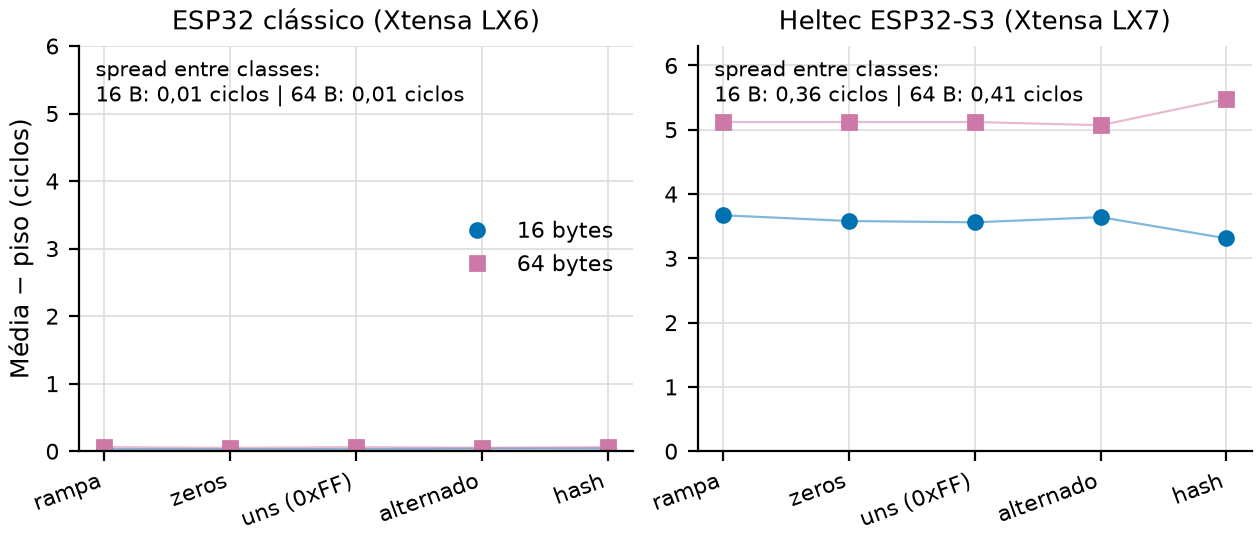
\includegraphics[width=\textwidth]{felipe/figuras/bench_tempo_constante.png}
  \end{center}
  \legend{Fonte: elaborado pelos autores.}
\end{figure}

%%%%%%%%%%%%%%%%%%%%%%%%%%%%%%%%%%%%%%%%%%%%%%%%%%%%%%

\subsection{Comparativo com AES-128-GCM}
\label{subsec:comparativo_aes}

Para responder à questão central levantada na Seção 2.2.2, se a migração para criptografia leve em \textit{software} traz vantagem real frente ao acelerador de \textit{hardware} já presente nas placas comerciais, comparou-se o Ascon-128a (\textit{software}) com o AES-128-GCM (\textit{Galois/Counter Mode}) na mesma execução e sob as mesmas condições, nas duas placas. O AES-GCM foi avaliado por meio da biblioteca \textit{mbedTLS} do próprio \textit{core} do ESP32, com a chave fixada uma vez por execução, como num nó que possui uma única chave. Nos dois chips, apenas o bloco AES é executado no acelerador de \textit{hardware}. A autenticação (GHASH) permanece em \textit{software}, e nenhum dos dois declara suporte a GCM no acelerador \cite{espressif2026idf}. As placas diferem no caminho pelo qual o \textit{driver} alimenta o acelerador. No ESP32 clássico a CPU escreve e lê um bloco de 16 bytes por vez, e no ESP32-S3 o \textit{driver} usa DMA \cite{espressif2026idf}.

Cada algoritmo foi medido pelo piso de 2.000 medidas, alternando-se os dois na mesma execução, em 100 execuções por tamanho, para cifragem e decifragem. A Tabela~\ref{tab:comparativo_aes} apresenta os pisos da cifragem e a razão entre eles, e a Tabela~\ref{tab:comparativo_aes_dec} faz o mesmo para a decifragem. A decifragem interessa por conta própria, pois é a operação que o receptor executa para cada pacote de cada nó. A Figura~\ref{fig:bench_ciclos_tamanho} mostra as mesmas curvas, com a cifragem acima e a decifragem abaixo.

\begin{table}[htb]
\centering
\caption{Piso de ciclos da cifragem do Ascon-128a (\textit{software}) e do AES-128-GCM (\textit{mbedTLS}), nas duas placas, e razão AES/Ascon}
\label{tab:comparativo_aes}
\begin{tabular}{rrrrrrr}
\hline
\textbf{\textit{Payload}} & \multicolumn{3}{c}{\textbf{ESP32 clássico}} & \multicolumn{3}{c}{\textbf{ESP32-S3}} \\
 & \textbf{Ascon} & \textbf{AES-GCM} & \textbf{razão} & \textbf{Ascon} & \textbf{AES-GCM} & \textbf{razão} \\
\hline
0 bytes  & 5.037 & 6.497  & 1,29 & 4.603 & 10.465 & 2,27 \\
2 bytes  & 5.181 & 8.174  & 1,58 & 4.722 & 16.556 & 3,51 \\
16 bytes & 6.134 & 8.603  & 1,40 & 5.639 & 19.473 & 3,45 \\
23 bytes & 6.521 & 10.454 & 1,60 & 5.960 & 20.920 & 3,51 \\
32 bytes & 7.231 & 10.712 & 1,48 & 6.675 & 20.398 & 3,06 \\
64 bytes & 9.425 & 14.930 & 1,58 & 8.747 & 22.267 & 2,55 \\
\hline
\end{tabular}
\legend{Fonte: elaborado pelos autores.}
\end{table}

\begin{table}[htb]
\centering
\caption{Piso de ciclos da decifragem do Ascon-128a (\textit{software}) e do AES-128-GCM (\textit{mbedTLS}), nas duas placas, e razão AES/Ascon}
\label{tab:comparativo_aes_dec}
\begin{tabular}{rrrrrrr}
\hline
\textbf{\textit{Payload}} & \multicolumn{3}{c}{\textbf{ESP32 clássico}} & \multicolumn{3}{c}{\textbf{ESP32-S3}} \\
 & \textbf{Ascon} & \textbf{AES-GCM} & \textbf{razão} & \textbf{Ascon} & \textbf{AES-GCM} & \textbf{razão} \\
\hline
0 bytes  & 5.256  & 6.908  & 1,31 & 4.755 & 10.814 & 2,27 \\
2 bytes  & 5.366  & 8.585  & 1,60 & 4.841 & 16.903 & 3,49 \\
16 bytes & 6.646  & 9.014  & 1,36 & 5.959 & 19.820 & 3,33 \\
23 bytes & 6.989  & 10.867 & 1,55 & 6.212 & 21.269 & 3,42 \\
32 bytes & 8.036  & 11.123 & 1,38 & 7.163 & 20.745 & 2,90 \\
64 bytes & 10.816 & 15.341 & 1,42 & 9.571 & 22.616 & 2,36 \\
\hline
\end{tabular}
\legend{Fonte: elaborado pelos autores.}
\end{table}

\begin{figure}[htb]
  \caption{\label{fig:bench_ciclos_tamanho}Piso de ciclos da cifragem (acima) e da decifragem (abaixo) por tamanho de \textit{payload}, Ascon-128a e AES-128-GCM, nas duas placas}
  \begin{center}
      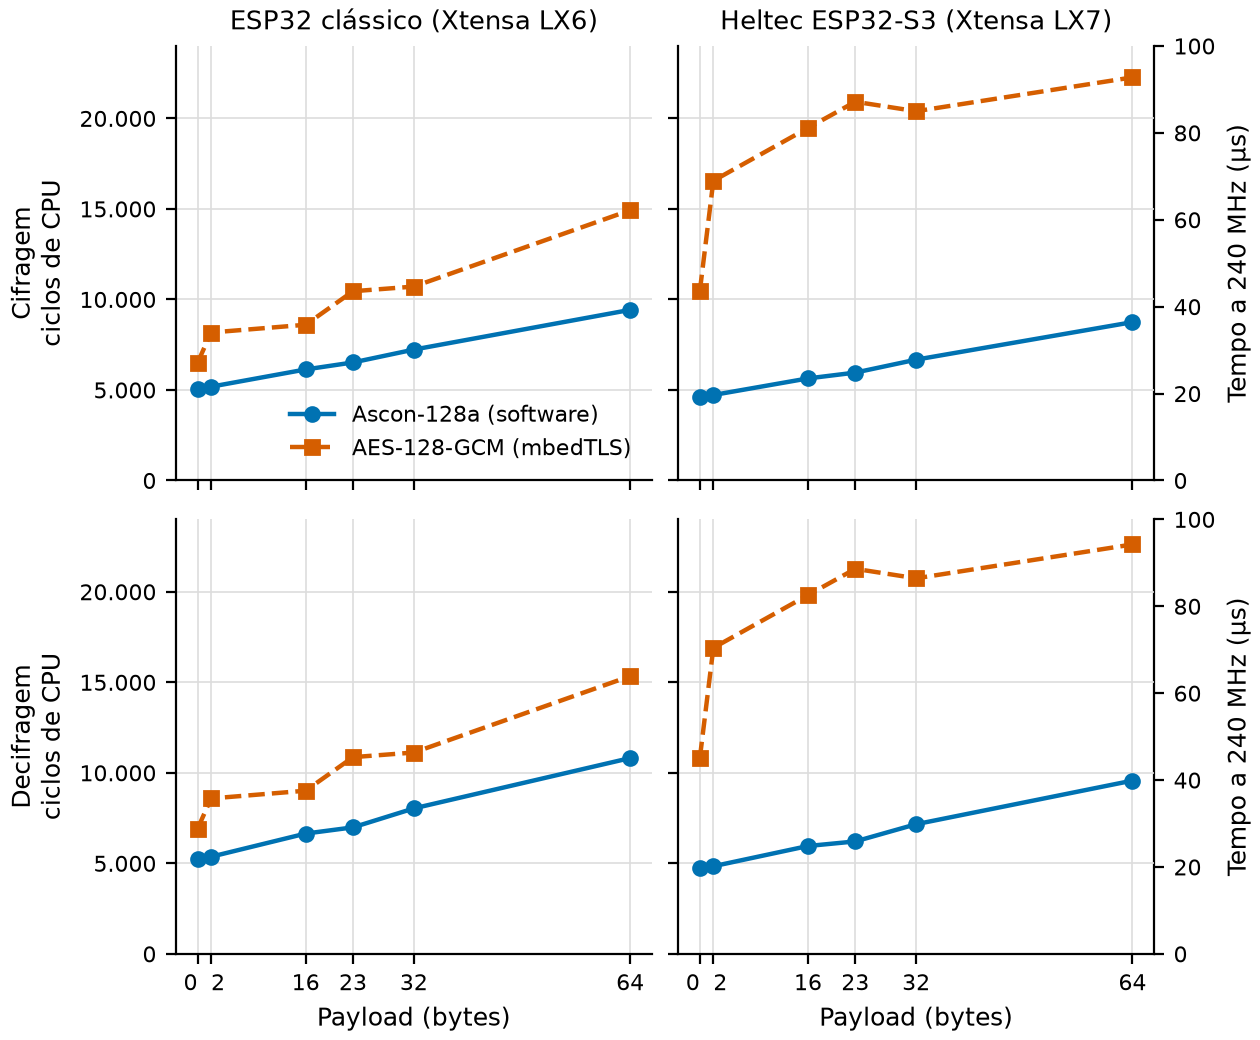
\includegraphics[width=\textwidth]{felipe/figuras/bench_ciclos_tamanho.png}
  \end{center}
  \legend{Fonte: elaborado pelos autores.}
\end{figure}

O Ascon-128a foi mais rápido que o AES-128-GCM em todas as 1.200 execuções de cada placa (seis tamanhos, cifragem e decifragem, 100 execuções). No ESP32 clássico a vantagem vai de 1,29 vez, com o \textit{payload} vazio, a 1,60 vez, em 23 bytes, e tende a crescer com o número de blocos. Na decifragem, vai de 1,31 a 1,60. No ESP32-S3 ela vai de 2,27 a 3,51 vezes na cifragem e de 2,27 a 3,49 na decifragem, e diminui com o tamanho (Figura~\ref{fig:bench_razao_tamanho}). As duas tendências têm a mesma origem, o custo por bloco e a parcela fixa de cada caminho do AES, examinados a seguir.

\begin{figure}[htb]
  \caption{\label{fig:bench_razao_tamanho}Razão entre os pisos de ciclos do AES-128-GCM e do Ascon-128a, na cifragem e na decifragem, por tamanho de \textit{payload}}
  \begin{center}
      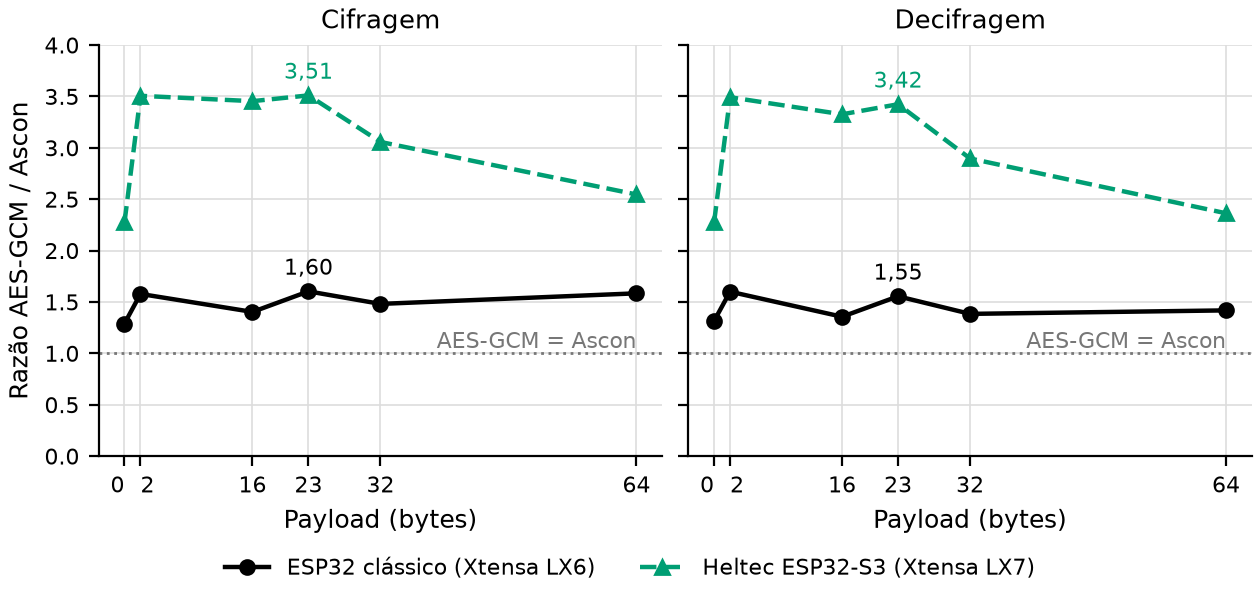
\includegraphics[width=\textwidth]{felipe/figuras/bench_razao_tamanho.png}
  \end{center}
  \legend{Fonte: elaborado pelos autores.}
\end{figure}

O AES-GCM é a cifragem em modo contador (CTR) mais o cálculo da \textit{tag} pelo GHASH \cite{dworkin2007gcm}, e no ESP-IDF a rotina de GCM reutiliza a de CTR \cite{espressif2026idf}. Assim, a diferença entre os custos por bloco dos dois modos é o GHASH, e por isso mediu-se também o AES-128-CTR. Ele entra aqui só como instrumento de medição, pois sem autenticação não atenderia ao requisito desta camada. A Figura~\ref{fig:bench_decomposicao_bloco} resume a decomposição. No ESP32 clássico, cada bloco adicional de 16 bytes custa 825 ciclos no AES-CTR e 2.109 no AES-GCM, logo 1.284 ciclos no GHASH. No ESP32-S3, são 49 ciclos no CTR, 931 no GCM e 882 no GHASH. Em ambos, o GHASH sozinho custa mais do que o Ascon-128a gasta para cifrar e autenticar um bloco inteiro (1.097 e 1.036 ciclos). Mesmo os 825 ciclos por bloco do CTR no ESP32 clássico estão longe do núcleo do acelerador, ao qual o manual do fabricante atribui 11 a 15 ciclos de \textit{clock} por bloco \cite{espressif2026trm}. O restante é gasto pelo \textit{software} do \textit{driver} e pela transferência dos dados entre a CPU e o periférico.

\begin{figure}[htb]
  \caption{\label{fig:bench_decomposicao_bloco}Custo marginal por bloco de 16 bytes do Ascon-128a completo e do AES-128-GCM decomposto em cifra AES (CTR) e GHASH, nas duas placas}
  \begin{center}
      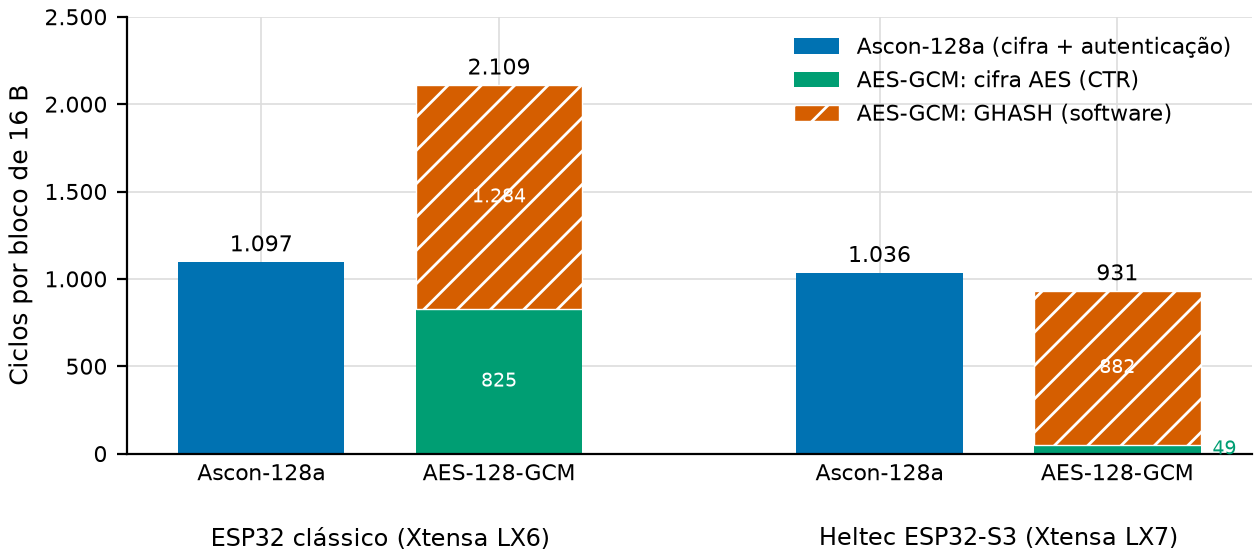
\includegraphics[width=\textwidth]{felipe/figuras/bench_decomposicao_bloco.png}
  \end{center}
  \legend{Fonte: elaborado pelos autores.}
\end{figure}

No ESP32-S3, o caminho por DMA reduz o custo por bloco a 49 ciclos, mas cobra caro por chamada. Cada transferência exige preparar e depois liberar o canal de DMA \cite{espressif2026idf}, e o AES-CTR de 16 bytes custou 8.218 ciclos, contra 2.316 no ESP32 clássico. Como o GCM faz duas transferências por mensagem, uma para os dados e outra para a \textit{tag}, sua parcela fixa chega a cerca de 18.500 ciclos, e é isso que torna o AES-GCM 3,5 vezes mais lento que o Ascon na mensagem de 23 bytes. O bloco parcial recebe tratamento à parte no \textit{driver}, o que ajuda a explicar 23 bytes terem custado mais que 32 (20.920 contra 20.398 ciclos). Os pisos do AES-GCM no ESP32-S3 variaram até 8 ciclos entre as 100 execuções, cerca de 0,04\%, e no ESP32 clássico no máximo 2. Os do Ascon não variaram em nenhum caso.

Para os pacotes pequenos típicos de redes LoRaWAN, portanto, a criptografia leve em \textit{software} não apenas dispensa o acelerador de \textit{hardware} como o supera em latência nos dois chips, e por margem maior justamente na placa de implantação, mantendo ainda a ausência de alocação dinâmica, que o AES não mantém no ESP32-S3. Ressalva-se que o resultado se refere ao AES-GCM do \textit{mbedTLS} pelo \textit{port} da Espressif, nas versões indicadas. Entre os alvos do ESP-IDF, apenas o ESP32-S2 declara aceleração de GCM, e ainda assim parcial, pois o GHASH permanece em \textit{software}, de modo que não se espera que a comparação se inverta nas demais variantes \cite{espressif2026idf}. O consumo energético dessa mesma comparação é apresentado na Seção~\ref{subsec:energia_resultados}.

%%%%%%%%%%%%%%%%%%%%%%%%%%%%%%%%%%%%%%%%%%%%%%%%%%%%%%

\subsection{Consumo Energético}
\label{subsec:energia_resultados}

A energia por operação foi medida pelo procedimento da Seção~\ref{subsec:energia_metodo}, nas duas placas, com a mensagem de 23 bytes. Um \textit{firmware} próprio, que executa um autoteste antes de começar, repetiu cada operação 20.000 vezes por rajada. Os cinco casos foram a cifragem e a decifragem do Ascon-128a e do AES-128-GCM e o controle, em que o processador apenas aguarda 27~$\mu$s por repetição. O resistor foi de 1~$\Omega$, com tolerância de 1\%. A tensão na placa foi medida com multímetro no ESP32-S3, 3,2~V, e não foi medida no ESP32 clássico, para o qual se adotou 3,25~V. O \textit{firmware}, as leituras e as capturas de tela do osciloscópio estão na pasta \texttt{benchmark-validation/Ascon128a\_Energy\_Burst} do repositório.

No ESP32 clássico, a média da rajada e a do repouso foram lidas na mesma captura, como previsto. No ESP32-S3, o osciloscópio calculou a média entre cursores apenas no instante da captura, e as duas médias vieram de capturas distintas, com os cursores fixados antes do disparo. Como o repouso é o mesmo estado da placa em todos os casos, adotou-se para cada placa um único valor, a média das cinco leituras de repouso, 49,0~mV no ESP32 clássico e 43,1~mV no ESP32-S3. Essas leituras variaram de 48,0 a 52,1~mV na primeira placa e de 42,0 a 46,2~mV na segunda, com desvio padrão de 1,7 e 1,8~mV. O acréscimo de corrente tem, portanto, incerteza de cerca de 2~mA, entre 7\% e 9\% do valor nos quatro casos com algoritmo. A Tabela~\ref{tab:energia_ascon128a} apresenta os resultados.

\begin{table}[htb]
\centering
\caption{Duração da rajada de 20.000 operações, acréscimo de corrente sobre o repouso e energia por operação, com mensagem de 23 bytes, nas duas placas}
\label{tab:energia_ascon128a}
\begin{tabular}{lrrrrrr}
\hline
\textbf{Caso} & \multicolumn{3}{c}{\textbf{ESP32 clássico}} & \multicolumn{3}{c}{\textbf{ESP32-S3}} \\
 & \textbf{s} & \textbf{mA} & \textbf{$\mu$J} & \textbf{s} & \textbf{mA} & \textbf{$\mu$J} \\
\hline
Controle                 & 0,55 & 12,6 & 1,1 & 0,556 & 19,8 & 1,8 \\
Ascon-128a, cifragem     & 0,52 & 25,1 & 2,1 & 0,499 & 28,1 & 2,2 \\
Ascon-128a, decifragem   & 0,57 & 25,6 & 2,4 & 0,520 & 27,9 & 2,3 \\
AES-128-GCM, cifragem    & 1,02 & 22,4 & 3,7 & 1,756 & 27,9 & 7,8 \\
AES-128-GCM, decifragem  & 1,05 & 22,5 & 3,8 & 1,786 & 25,9 & 7,4 \\
\hline
\end{tabular}
\legend{Fonte: elaborado pelos autores.}
\end{table}

O Ascon-128a gastou entre 2,1 e 2,4~$\mu$J por operação, nas duas placas. O AES-128-GCM gastou 3,7 e 3,8~$\mu$J no ESP32 clássico, 1,8 e 1,6 vez a energia do Ascon na cifragem e na decifragem, e 7,8 e 7,4~$\mu$J no ESP32-S3, 3,5 e 3,2 vezes. Essas razões carregam a incerteza de cada medida.

A diferença vem do tempo, e não da potência. Durante a rajada os dois algoritmos acrescentaram correntes próximas, de 22 a 28~mA, e no ESP32-S3 praticamente iguais na cifragem, 28,1 e 27,9~mA. O que muda é a duração. No ESP32-S3 cada operação do AES-128-GCM durou 87,8~$\mu$s e cada operação do Ascon-128a, 24,9~$\mu$s, a mesma razão de 3,5 vezes medida em ciclos na Tabela~\ref{tab:comparativo_aes}, cuja origem é a parcela fixa do caminho por DMA discutida na Seção~\ref{subsec:comparativo_aes}. O caso de controle mostra que manter o núcleo ocupado, sem algoritmo algum, já acrescenta 12,6~mA no ESP32 clássico e 19,8~mA no ESP32-S3. O Ascon acrescenta a isso cerca de 13~mA na primeira placa e 8~mA na segunda.

As durações das rajadas foram comparadas com os pisos de ciclos das seções anteriores, multiplicados pelas 20.000 repetições. No ESP32-S3, em que a duração foi medida pelo próprio osciloscópio, as quatro ficaram a menos de 1\% do previsto, com 0,499~s contra 0,497~s na cifragem do Ascon e 1,756~s contra 1,743~s na do AES-GCM. No ESP32 clássico, em que foi lida pelos cursores com resolução de 0,03~s, as do Ascon ficaram dentro dessa margem. As do AES-GCM duraram 1,02 e 1,05~s, contra 0,87 e 0,91~s previstos. A causa dessa diferença não foi investigada, e a energia foi calculada com a duração medida.

%%%%%%%%%%%%%%%%%%%%%%%%%%%%%%%%%%%%%%%%%%%%%%%%%%%%%%

\subsection{Integração no enlace LoRa: biblioteca \textit{AsconSecure}}
\label{subsec:asconsecure}

As seções anteriores validam o algoritmo. Para que a frente de comunicação o utilize sem lidar com chave, \textit{nonce} ou contador, a camada de segurança foi empacotada como uma biblioteca Arduino, a \textit{AsconSecure}, na pasta \texttt{ascon-lora} do repositório. Ela reúne três papéis. O provisionamento do nó é feito uma vez na bancada, o emissor cifra no nó sensor, e o receptor decifra no \textit{gateway}. Para a aplicação, o uso se resume a uma chamada para cifrar e uma para decifrar. Quando a operação falha, o resultado não contém bytes, e não há o que transmitir ou consumir.

Cada mensagem no ar é formada por um contador de 4 bytes, pelo texto cifrado e pela \textit{tag} de 16 bytes, o que acrescenta 20 bytes fixos ao \textit{payload}. O \textit{nonce} de 128 bits é composto por um prefixo de 12 bytes, gerado no provisionamento e conhecido pelo receptor, seguido do contador, e só o contador viaja. Ele não precisa de proteção à parte, pois alterá-lo em trânsito altera o \textit{nonce} e invalida a \textit{tag}, como mostrou a Seção~\ref{subsec:aead_resultados}.

A chave de 128 bits e o prefixo são gerados no próprio nó, pelo CTR\_DRBG da \textit{mbedTLS} alimentado pelo gerador de \textit{hardware} do ESP32 (RF-S3 e RF-S4), e gravados na memória não volátil (NVS). A saída do gerador é usada diretamente como chave, o caso $V$ nulo da operação $K = U \oplus V$ do SP 800-133r2 \cite{barker2020nist133}. Um cuidado vem da documentação do ESP-IDF. O gerador de \textit{hardware} só produz números verdadeiramente aleatórios com o Wi-Fi ou o Bluetooth ligados, ou com uma fonte interna de entropia habilitada por \texttt{bootloader\_random\_enable()}, e fora dessas condições sua saída deve ser considerada apenas pseudoaleatória \cite{espressif2026random}. Como o nó não usa Wi-Fi nem Bluetooth, a biblioteca habilita essa fonte durante a geração da chave e a desabilita em seguida. A mesma documentação exige que isso ocorra antes de o conversor analógico-digital ou o rádio serem iniciados, e por isso a geração da chave é uma etapa própria, o provisionamento, separada da inicialização do emissor. Como cada nó gera a própria chave, nenhuma é compartilhada (RF-S6), e o \textit{gateway} não tem chave própria, apenas guarda a de cada nó que escuta.

A unicidade do \textit{nonce} (RNF-S2 e RF-S7) vem de um contador de 32 bits persistido na NVS. Para não gravar a \textit{flash} a cada mensagem, o emissor reserva 32 valores por vez, gravando o valor 32 posições à frente antes de usar a faixa, e só volta a gravar quando ela se esgota. Após uma reinicialização, o contador recomeça do valor reservado, pois tudo abaixo dele pode ter ido ao ar. Uma queda de energia descarta até 32 valores, mas nunca repete um, e diante de $2^{32}$ valores o descarte é irrelevante. O contador pertence a esta camada e independe do contador de quadros do LoRaWAN, como exige o RF-S7. Perto do fim, a cifragem é recusada antes que o valor dê a volta, e a saída é reprovisionar o nó.

No \textit{gateway}, o receptor guarda na NVS, para cada nó, o maior contador já aceito. A decifragem verifica primeiro a \textit{tag} e depois o contador. Um pacote com \textit{tag} inválida é descartado antes de qualquer consulta ao estado, para que um pacote forjado com contador alto não bloqueie o nó legítimo, e um pacote autêntico com contador igual ou menor que o último aceito é descartado como repetição (RF-S9). O novo contador é gravado antes de a mensagem ser entregue. Se a gravação falhar, a mensagem é descartada, pois entregar sem gravar permitiria, após um reinício, aceitar de novo tudo o que chegou no intervalo. O texto claro fica num \textit{buffer} interno e só é copiado à aplicação depois das duas verificações, o que estende ao código de integração a garantia do RF-S8. O registro é indexado por uma impressão da chave, os 8 primeiros bytes do \textit{hash} Ascon de chave e prefixo, e não pelo número do nó, para que um erro de configuração, como registrar o mesmo nó sob dois números, não reabra o histórico à repetição.

A renovação da chave (RF-S5) é feita por novo provisionamento, em que se apaga o estado do nó, gera-se nele uma chave nova e substitui-se o registro no receptor. Nenhuma chave trafega pelo ar.

Os \textit{buffers} da biblioteca têm tamanho fixo e a cifragem não aloca memória dinâmica, como medido na Seção~\ref{subsec:memoria_tempo}. O tamanho máximo do \textit{payload} é uma constante de compilação da biblioteca, de 200 bytes na configuração padrão, ajustável conforme o projeto. O acesso à NVS, feito pelo ESP-IDF, cria e libera um objeto em memória dinâmica a cada gravação \cite{espressif2026idf}, isso ocorre fora da cifragem, uma vez a cada 32 mensagens no emissor e a cada mensagem aceita no receptor. A Tabela~\ref{tab:asconsecure_requisitos} resume o atendimento aos requisitos da Seção~\ref{sec:requisitos_seguranca}.

\begin{table}[htb]
\centering
\caption{Requisitos da Seção~\ref{sec:requisitos_seguranca} atendidos pela biblioteca \textit{AsconSecure}}
\label{tab:asconsecure_requisitos}
\begin{tabular}{lp{10cm}}
\hline
\textbf{Requisito} & \textbf{Como é atendido} \\
\hline
RF-S2, RF-S3, RF-S4 & Chave gerada no nó pelo CTR\_DRBG da \textit{mbedTLS}, semeado pelo gerador de \textit{hardware} com a fonte interna de entropia habilitada, com $V$ nulo. \\
RF-S5           & Renovação por novo provisionamento, nenhuma chave trafega pelo ar. \\
RF-S6           & Cada nó gera a própria chave e o \textit{gateway} guarda uma por nó. \\
RF-S7           & Contador de 32 bits na NVS, reservado em blocos de 32 antes do uso, independente do contador de quadros do LoRaWAN. \\
RF-S8           & Texto claro só é copiado à aplicação após \textit{tag} e contador aprovados. \\
RF-S9           & Receptor descarta contador igual ou menor que o último aceito, gravado antes da entrega. \\
RNF-S1          & Entropia bruta condicionada pelo CTR\_DRBG. \\
RNF-S2          & Chave guardada na NVS do nó e apagada da RAM ao ser descartada, e \textit{nonce} único pelo contador. \\
RNF-S5          & \textit{Tag} de 16 bytes, sem truncamento. \\
RNF-S6, RNF-S7    & \textit{Buffers} de tamanho fixo e cifragem sem alocação dinâmica. \\
\hline
\end{tabular}
\legend{Fonte: elaborado pelos autores.}
\end{table}

Dois limites ficam registrados. O provisionamento imprime a chave na porta serial para ser copiada ao receptor, o que só é aceitável na bancada, com o nó sob controle físico. E o registro anti-repetição vive na NVS do \textit{gateway}. Se ela for apagada, mensagens antigas voltam a ser aceitas, cada uma no máximo uma vez, até que o contador do nó legítimo as ultrapasse. A execução da biblioteca no enlace, com nó e \textit{gateway} em operação, foi feita pela frente de infraestrutura e está relatada na Seção~\ref{sec:resultados_infra}.

%%%%%%%%%%%%%%%%%%%%%%%%%%%%%%%%%%%%%%%%%%%%%%%%%%%%%%

\subsection{Limitações das Medições}
\label{subsec:limitacoes_ascon}

O atendimento de cada requisito da Seção~\ref{sec:requisitos_seguranca} está resumido na Tabela~\ref{tab:rastreabilidade_ascon}. Os resultados desta seção valem para as condições em que foram obtidos. As placas foram o ESP32 clássico e o ESP32-S3 da Heltec, a 240~MHz, com o \textit{core} arduino-esp32 3.3.11 sobre o ESP-IDF 5.5.5 e a biblioteca \textit{ascon-suite} na versão indicada na Seção~\ref{subsec:biblioteca-ascon}. Nada aqui se generaliza para outras famílias de microcontroladores, e o próprio fabricante observa que a 240~MHz o acelerador de AES não oferece ganho sobre o AES em \textit{software} \cite{espressif2026idf}, o que faz parte do contexto da comparação. A variante medida é o Ascon-128a versão 1.2, e não o Ascon-AEAD128 do SP 800-232, cujas diferenças se limitam a constantes, como mostra a Tabela~\ref{tab:parametros_ascon}. Os \textit{payloads} foram de 0 a 64 bytes, o modelo linear de custo foi validado nessa faixa e não foi verificado para mensagens maiores. A resistência a canais laterais foi avaliada apenas quanto ao tempo de execução, consumo de potência e emissão eletromagnética ficam como trabalho futuro. A energia por operação foi medida apenas para a mensagem de 23 bytes, com uma captura por leitura, e não inclui o rádio. No ESP32 clássico a tensão na placa foi adotada, e não medida. O tempo no ar é calculado pela fórmula do fabricante do rádio, não medido. O subconjunto do KAT foi executado em placa apenas no ESP32 clássico, e no ESP32-S3 a correção foi verificada pelos dois vetores que o \textit{firmware} de medição executa antes de começar. Por fim, a camada foi avaliada fora de uma rede LoRaWAN completa, de modo que a proteção da camada MAC do LoRaWAN não faz parte do que foi medido.
